\begin{blocksection}
\question
\textbf{among us}\\
Fill in each blank in the code example below so that its environment diagram is the following. You do not need to use all the blanks.

\begin{multicols}{2}
\begin{lstlisting}
def among(green):
    def us(yellow):
        _____________________
        yellow += ___________
        green += ____________
        _____________________
        return ______________
    return ______________
vote = among('Red')('Blue')()
\end{lstlisting}


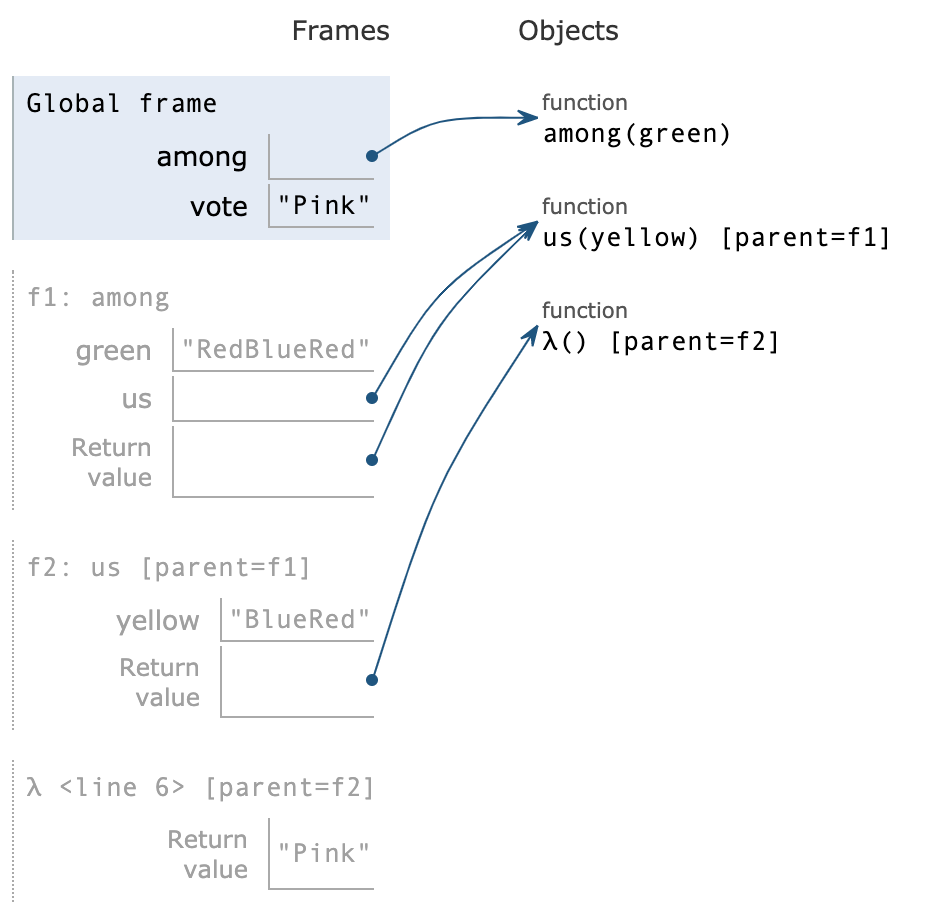
\includegraphics[width=.5\textwidth]{amongus.png}
\end{multicols}

\begin{solution}[2in]
\begin{lstlisting}
def among(green):
    def us(yellow):
        nonlocal green
        yellow += green
        green += yellow
        return lambda : 'Pink'
    return us
vote = among('Red')('Blue')()
\end{lstlisting}
\end{solution}
\end{blocksection}

\begin{blocksection}
\begin{guide}
\textbf{Teaching Tips}
\begin{itemize}
\item Highlight the multiple higher-order functions that come into play in this problem. Take note of how none of the function assignments seem to change in the environment diagram, which means we don't have to worry about manipulating the functions themselves in this problem.
\item What's a common return value for the functions in these types of HOF problems? Returning the inner function itself (or a lambda function!).
\item Go left to right for each function call (top to bottom in the environment diagram). Two good steps to do each time we step into a function are to check the value of its input(s) and its return value(s); those tell us a lot about what kind of manipulations we do inside the function.
\item Pay careful attention to the scope of each variable! Each time you change or reassign a variable, think about if you are allowed to do so in your current frame. If not, what can you add to make that possible?
\end{itemize}
\end{guide}
\end{blocksection}
